\documentclass[11pt,letterpaper]{article}
\usepackage[T1]{fontenc}
\usepackage{lmodern,microtype,amsmath,amssymb,booktabs,graphicx,xcolor}
\usepackage[top=.81in,bottom=.84in,left=.89in,right=.89in,headheight=14pt,headsep=14pt,footskip=26pt]{geometry}
\usepackage{fancyhdr,titlesec}
\usepackage[colorlinks=true,allcolors=teal!55!black]{hyperref}
\definecolor{ink}{HTML}{1D3842}
\definecolor{tealink}{HTML}{11696D}
\definecolor{paleteal}{HTML}{E8F3F0}
\titleformat{\section}{\Large\sffamily\bfseries\color{ink}}{\thesection}{.6em}{}
\titlespacing*{\section}{0pt}{14pt}{7pt}
\titleformat{\paragraph}[runin]{\bfseries\color{ink}}{}{0pt}{}
\titlespacing*{\paragraph}{0pt}{7pt}{.65em}
\setlength{\parindent}{0pt}\setlength{\parskip}{3.6pt plus 1pt minus .7pt}
\setlength{\emergencystretch}{2em}
\setlength{\abovedisplayskip}{7pt plus 2pt}\setlength{\belowdisplayskip}{7pt plus 2pt}
\pagestyle{fancy}\fancyhf{}
\fancyhead[L]{\sffamily\small\color{ink} Convex covers of unit space curves}
\fancyhead[R]{\sffamily\small\color{ink} 20 November 2026}
\fancyfoot[R]{\sffamily\small\color{ink}\thepage}
\renewcommand{\headrulewidth}{.25pt}\raggedbottom
\hypersetup{pdftitle={Sharper volume bounds for a convex cover of every unit space curve},pdfauthor={OpenAI}}
\begin{document}
\thispagestyle{plain}
{\small\sffamily\color{tealink} CONVEX GEOMETRY\hfill 20 NOVEMBER 2026\par}
\vspace{6pt}
{\fontsize{26}{29}\selectfont\sffamily\bfseries\color{ink}
Sharper bounds for convex covers\\of unit space curves\par}
\medskip
Let $V_3$ be the smallest volume of a convex body that can contain a rigid
copy of each smooth space curve of length one. Endpoints are free.
We prove that the minimum exists and satisfies
\begin{center}
\setlength{\fboxsep}{8pt}\colorbox{paleteal}{\makebox[.77\linewidth]{\large
$\displaystyle 0.01942 < V_3 < 0.052942305538.$}}
\end{center}
The lower bound uses three test paths. Project a candidate body along
its unit segment. Its shadow must fit a long chord forced by a planar
arc, together with some projection of a particular spatial arc. Even
after both can move, the shadow needs area greater than $0.05826$.

For the upper bound we give a rational polytope. Every unit curve fits a right
prism whose height controls the length of its planar projection. Allowing
the position and orientation of the prism to vary with height gives the
cover pictured below. Its exact volume is
\[
 \frac{13235576384310899273916967194112370723463873}
      {250000000000000000000000000000000000000000000}.
\]
This is the volume of the exhibited cover. The minimizing shape and exact
minimum remain undetermined.
\begin{center}
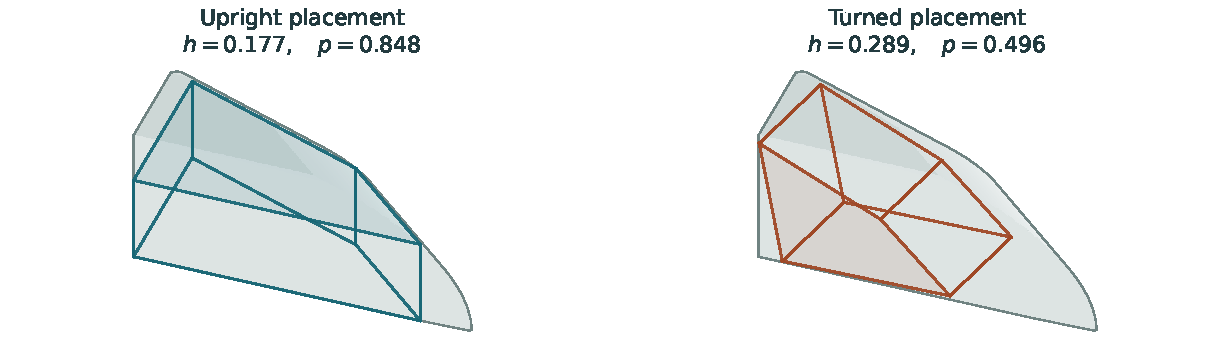
\includegraphics[width=.98\linewidth]{upper/adaptive_cover.pdf}
\end{center}
{\small Two complete prisms inside the same polytope, viewed from the
same direction. The original support planes are $h$ apart. The planar
projection fits a quadrilateral scaled by $p=\sqrt{1-9h^2}$.\par}
\medskip
\begin{center}
\begin{tabular}{@{}lrr@{}}
\toprule
& Lower endpoint & Upper endpoint\\\midrule
First linked report \cite{original} & $0.0187328127$ & $0.0542671$\\
Linked refinement \cite{refinement} & $0.018975$ & $0.052956040$\\
This work & $0.019420$ & $0.052942305538$\\\bottomrule
\end{tabular}
\end{center}
{\small The table uses outward bounds. All new numerical comparisons
are certified with integer or rational arithmetic.\par}
\clearpage
\section{Curves, rigid motions and attainment}\label{sec:setting}
A placement is $x\mapsto Rx+t$, where $R\in SO(3)$. The containing body
is compact and convex and may touch the curve. Length counts retracing.
A closed curve is allowed, and a segment with distinct endpoints is also
a test. Scaling space shows that the answer for length $L>0$ is $L^3V_3$.

\paragraph{Why a smooth-curve problem permits polygons.}
In fact the same bodies cover every rectifiable arc of length one.
Parametrize such an arc by arclength. Inscribed polygons can be chosen
with vanishing mesh and lengths tending to one: take partitions nearly
attaining total variation and refine them by a uniform mesh. Their images
converge in Hausdorff distance by uniform continuity. Perturb each finite
list of vertices by sufficiently small amounts to make links nonzero
and adjacent unit tangents nonopposite, with vanishing changes of length
and position along the sequence. Parametrize each polygon by its own
arclength and extend the end segments linearly. Convolve with a
nonnegative smooth kernel of integral one and support radius smaller than
half the shortest edge. Near a corner the new derivative is a convex
combination of the two adjacent unit tangents and is nonzero. Off the
corner neighborhoods it is the original unit tangent. For each polygon,
shrinking the kernel gives uniform convergence and convergence of length,
since the speed is at most one and the exceptional intervals have
vanishing total length. A final dilation about the first point gives
smooth regular arcs of length exactly one converging to the required
image. The kernel radius and the perturbations may be chosen separately
for each polygon. If simple smooth arcs are required, a general-position
perturbation in three dimensions makes nonadjacent edges disjoint.
Small corner neighborhoods can be chosen disjoint from other edges;
local injectivity during smoothing follows by strict monotonicity in
the direction of the sum of the two unit tangents.

Anchor the initial points at the origin. For any fixed candidate body
the translations in a fitting sequence then belong to that body, and
the rotations belong to compact $SO(3)$. A subsequence of motions
converges, placing the limiting curve inside the closed body. Every
shorter path may first be extended to length one. This argument also
explains why rounding the paths themselves need not preserve their
widths exactly.

\paragraph{Existence of a smallest body.}
The arclength midpoint lies within $1/2$ of every point, so the
radius-$1/2$ ball is universal. Three edges in succession visiting
all vertices of a regular tetrahedron of side $1/3$ form a unit path.
Every universal body contains a copy of the solid tetrahedron and
hence some fixed-radius ball of radius $r>0$. In a minimizing sequence,
translate each such ball to be centered at zero. For any point $x$ of
one of the bodies $K$, the cone on the radius-$r$ disk through zero
normal to $x$ has apex $x$ and lies in $K$. Hence
$\|x\|\le3|K|/(\pi r^2)$. All the bodies in the sequence lie in a
single ball.

For completeness, a Hausdorff-convergent subsequence can be selected
by recording which cubes of a finite mesh meet each body, stabilizing
this finite list on a subsequence, and diagonalizing over dyadic meshes.
Agreement on a mesh puts either set within its cube diameter of the
other. The limit consists of the subsequential limits of points from the
sets; compactness of the common bounding ball gives existence of these
limits and Hausdorff convergence. Convexity passes to the limit $K_*$,
as does inclusion of the fixed ball. At Hausdorff distance at most
$\delta$, either body lies in the other's concentric dilation by
$1+\delta/r$, since $K+\delta B_3\subset (1+\delta/r)K$ for
$rB_3\subset K$. Volumes therefore converge. For each fixed curve
extract a convergent subsequence of its placements as above. Its limit
lies in the already fixed $K_*$. Thus $K_*$ is universal and has the
infimal volume.
\section{Three paths force a large shadow}\label{sec:shadow}

Put $b=0.43892$. We use a straight unit segment, a planar polygonal arc
of minimum planar width greater than $b$, and a particular polygonal arc
$G$ in three dimensions. Each path can have its own rigid placement.
Throughout this section, area means two-dimensional Lebesgue measure.

\paragraph{Projection along the unit segment.}
Let $u$ be the direction of the segment in a universal body $K$ and
let $P$ be the orthogonal projection of $K$ onto $u^\perp$. The plane of
the placed planar arc contains a direction perpendicular to $u$. Projection
preserves its width in that direction, so $P$ has diameter greater than
$b$ and contains a straight chord of length $b$. Rotate horizontal
coordinates to make this chord parallel to the $x$-axis.

Write $\ell(y)$ for the length of the fiber of $K$ over $y\in P$.
The fiber over the projected unit segment $y_0$ has length at least one.
Joining both endpoints of that segment to one point over each $y$ gives
$\ell(ty_0+(1-t)y)\ge t$. Thus
\[
 |K|=\int_P\ell(y)\,dy
 \ge |P|\int_0^1(1-t)^2\,dt=\frac{|P|}{3}.
 \tag{1}\label{eq:fiber}
\]
Up to a translation, $P$ also contains an orthogonal projection of a
rotation of $G$. A translation of the whole picture lets us fix that
projection at the origin of our coordinate system and let the chord
translate freely. We will prove that every such planar convex set
has area greater than $0.05826$.

\paragraph{The two polygonal witnesses.}
The planar path's $69$ vertices are specified by the integer table and
reflection in \texttt{lower/check\_planar.py}. They sample the planar
caliper of Adhikari and Pitman \cite{caliper}. Divide the coordinates by
$2{,}278{,}289{,}034$, the sum of $1+\lfloor\sqrt{m}\rfloor$ over the
squared integer link lengths $m$. Its length is less than one. To bound its
width from below, test the normals to the differences of each of the $2346$
pairs of points. Between consecutive directions at which projections of
two vertices tie, the extreme vertices are fixed and the width $f(\theta)$
satisfies $f''=-f<0$. Its minimum is therefore at a tested endpoint.
For every pair the code squares and compares the integer projection span
with $b$ times the length of its normal, accounting for the denominator.
All tests are strict. This verifies the needed width directly.

The successive $61$ vertices of the spatial arc $G$ are the integer
triples in \texttt{lower/witness.hpp}, in units of $10^{-7}$. We obtained
them by deforming the inspection polygon of the linked refinement
\cite{refinement} to increase the area forced by its projections and the
chord. Their displayed integer coordinates are the definition of $G$.
Writing $F=\operatorname{conv}G$ and $B_3$ for the unit ball, the exact
checks give
\[
 L(G)<0.9999830,\qquad 0.102 B_3\subseteq F\subseteq 0.245 B_3 .
 \tag{2}\label{eq:balls}
\]
The length check uses the same integer square-root bound as above.
Checking the outer radius only needs squared vertex norms. Four affinely
independent vertices certify full dimension. Every facet plane of $F$
passes through a noncollinear triple, so enumerate all such triples.
If all vertices are on one side, choose the outward normal $n$ and
offset $s$. In the integer coordinates the program checks $s>0$ and
$s^2\ge 1{,}020{,}000^2\|n\|^2$ for each of the $118$ supporting
triples. Intersecting the facet half-spaces proves the inball claim.
The included script \texttt{lower/check\_witness.py} carries out these tests.
Shorter curves are legitimate by the closure argument in Section~\ref{sec:setting}.

\section{An area test with the chord free to move}\label{sec:planar}

For a compact convex set $D$ and vector $n$, write
$h_D(n)=\max_{v\in D}n\cdot v$. Given finitely many planar points known
to lie in the shadow, the following test bounds the area uniformly in the
position of the horizontal chord.

\noindent\begin{minipage}{\linewidth}
\centering
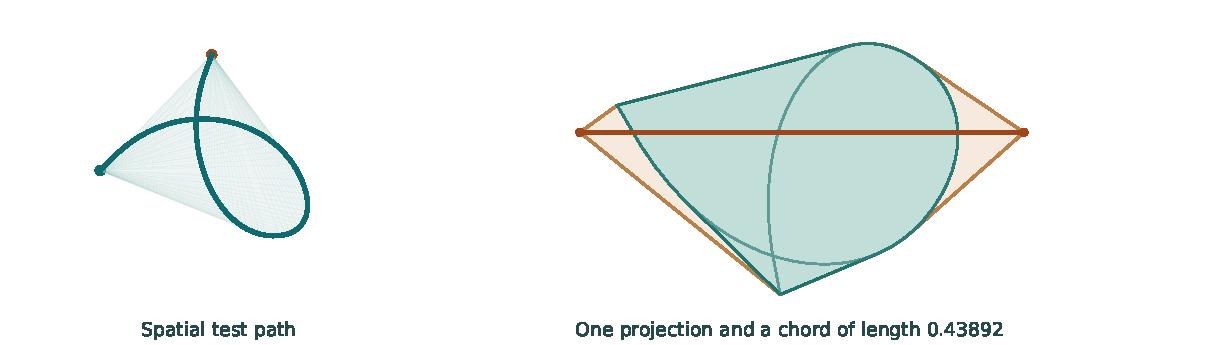
\includegraphics[width=.83\linewidth]{lower/shadow.pdf}\par
\raggedright\small
The planar picture shows one orthogonal shadow of the spatial witness and
one position of the compulsory chord. The orange boundary is their joint
convex hull. The proof allows every rotation of the path and every
translation of the chord.
\end{minipage}

\paragraph{Centering horizontal slices.}
Replace the intersection of a convex set with each horizontal line by an
interval of the same length centered on the $y$-axis. The result is
convex, because the interval length is a concave function of height:
interpolating two intervals gives a subinterval of the corresponding
intermediate slice. Fubini's theorem gives equality of areas, and inclusion
of sets is preserved. In particular the symmetrized shadow still contains
a chord of length $b$, now centered at $(0,c)$ for some unknown real $c$.

Let $Q$ be any polygon contained in the symmetrization of the known points'
convex hull. In the verifier all lengths at this stage are in units of
$10^{-6}$, so the chord length is the integer $d=438920$. Orient the
vertices $v_i$ of $Q$ counterclockwise. For an edge vector
$(\Delta x_i,\Delta y_i)$ put $n_i=(\Delta y_i,-\Delta x_i)$ and
$o_i=n_i\cdot v_i$. If a planar body $D$ contains $Q$ and a horizontal
segment of length $d$ centered at $(0,c)$, then
\[
 2|D|\ \ge\ 2|Q|+\sum_i
 \left[\frac{d}{2}|n_{ix}|+c\,n_{iy}-o_i\right]_+,
 \qquad [a]_+=\max(0,a).                         \tag{3}\label{eq:mix}
\]

\emph{Proof.} Let $M$ be the hull of $Q$ and the segment. For any two
convex polygons $Q,M$, the coefficient of $t$ in $|Q+tM|$ is
$\sum_i h_M(n_i)$. To see this, translate $M$ to contain zero. At
first order each edge sweeps a strip of length $\|n_i\|$ and width
$t h_M(n_i)/\|n_i\|$; the finitely many corner contributions have
area $O(t^2)$. Translation does not affect the sum since $\sum_i n_i=0$.
The edge list of $Q+tM$ is formed by merging the cyclic edge lists
of $Q$ and $tM$, since the face exposed by each normal is the sum of
the two exposed faces. Its starting vertex is likewise a sum. The
shoelace formula therefore makes $|Q+tM|$ a quadratic in $t$.
Its constant coefficient is $|Q|$, and its leading coefficient is
$|M|$ by rescaling and taking $t\to\infty$. Since $Q\subseteq M$,
we have $Q+tM\subseteq(1+t)M$. Cancelling the quadratic terms,
dividing by $t$ and letting $t\to\infty$ bounds the linear coefficient
by $2|M|$. Now $h_M(n_i)=\max(o_i,d|n_{ix}|/2+c n_{iy})$ and
$\sum_i o_i=2|Q|$. As $M\subseteq D$, this proves \eqref{eq:mix}.
\hfill$\square$

\paragraph{One-variable minimization.}
The right side of \eqref{eq:mix} is a convex piecewise-linear function
of $c$. On scaling the sum by two, its individual terms are
$[a_i+b_i c]_+$, where $a_i=d|n_{ix}|-2o_i$ and $b_i=2n_{iy}$.
The initial slope is $\sum_{b_i<0} b_i$ and each finite breakpoint
$-a_i/b_i$ contributes an upward jump of $|b_i|$. Sorting the rational
breakpoints and taking the first at which the accumulated slope is
nonnegative gives the global minimum, including a flat interval of
minimizers. Terms with $b_i=0$ are simply constants. Thus the test
eliminates every possible chord translation by integer comparisons.

For integer input points, compute the left and right boundary chains of
their hull in order of increasing height. At every vertex height
interpolate both endpoints of the horizontal slice and round its
half-length down to an integer. Take the hull of the resulting pairs of
opposite slice endpoints to form $Q$. Each pair is in the centered
slice, so all these inward roundings preserve \eqref{eq:mix}. The chain
algorithm discards the middle of any successive triple that bends in the wrong direction for the required chain. The lower convex and upper concave envelopes in coordinates $(y,x)$ thus give the two slice endpoints. Even omitting interior heights would only shrink the polygon used for the lower bound.

\section{A finite proof for every rotation}\label{sec:rotation}

We describe the coverage of the rotation group and the error estimate
explicitly. The only inputs to the loop are the integer vertices, the
chord length, the bounds in \eqref{eq:balls}, and the claimed area
threshold. There is no stored list of successful rotations.

Identify a rotation with quaternion conjugation by a nonzero
quaternion $q=(q_0,q_1,q_2,q_3)$, normalized by $\|q\|^2$.
Every proper rotation has such a representation: a rotation of angle
$\theta$ about a unit axis $u$ is represented by
$\cos(\theta/2)+u\sin(\theta/2)$. Left multiplication by one of
$1,i,j,k$ can move a component of largest magnitude into the scalar
position. On rotated vectors this just applies a coordinate half-turn,
so the projected figure changes at most by signs of its two coordinates.
Area and the constraint on a horizontal unoriented chord are preserved.
Rescale the quaternion to put its scalar component equal to $1$.
It suffices to check the single parameter cube $(q_1,q_2,q_3)\in[-1,1]^3$.

\paragraph{A polygon valid on an entire cell.}
At subdivision depth $k$ put $m=2^k$. In homogeneous integer coordinates
the center quaternion is $q=(m,v_1,v_2,v_3)$, with each free coordinate
of any other quaternion $q'$ in the cell differing by at most one.
Let $L$ be the floor of
\[
 \sqrt{m^2+\sum_{j=1}^3 \max(0,|v_j|-1)^2}.
\]
Both quaternion lengths are at least $L$. Their unit representatives
differ by at most $\sqrt3/L$. Indeed for nonzero $a,b$,
\[
 \|a-b\|^2=(\|a\|-\|b\|)^2+
  \|a\|\|b\|\left\|a/\|a\|-b/\|b\|\right\|^2 .
\]
For unit quaternions $s,t$, write $s x\bar s-t x\bar t$ as
$(s-t)x\bar s+t x(\bar s-\bar t)$. Its norm is at most
$2\|s-t\|\|x\|$. Thus, in units of $10^{-6}$, every projected vertex
moves by at most
\[
 \varepsilon=\lceil849000/L\rceil,
 \qquad 2\sqrt3\,245000<849000.
\]
If the center's vertical projection span, less $2\varepsilon$, is $s$,
then the true transverse span is at least $s$. Taking triangles on the
horizontal chord from the two transverse extremes of the entire planar
container gives twice-area at least $ds$. The chord lies between those
extremes and the two triangle interiors are disjoint. This yields a
quick test when $ds$ exceeds the threshold. Otherwise form a common
inner polygon as follows.

Write $B_0$ for the projected hull at the center and $B$ for the true
projected hull at any parameter in the cell. For every unit planar $n$,
$h_{B_0}(n)\le h_B(n)+\varepsilon$ and $h_B(n)\ge r=102000$ in
these units. Scale every center projection by
$\alpha=(r-2)/(r+\varepsilon)$ and truncate both coordinates towards
zero to integers. Each rounding error has norm less than $2$. For the
hull $J$ of the resulting points,
\[
 h_J(n)\le \alpha(h_B(n)+\varepsilon)+2\le h_B(n).
\]
The last inequality follows by substituting $h_B(n)\ge r$. A point outside a compact convex set is strictly separated by the line through its nearest point perpendicular to the joining segment. The support inequalities thus give $J\subseteq B$ throughout the cell.
The area test of Section~\ref{sec:planar} can therefore use $J$.

\paragraph{Exhaustion and exact arithmetic.}
Start at $(m,v)=(1,0)$. If neither the span nor the polygon test proves
the claimed strict inequality, replace the cell by its eight children
$(2m,2v+\sigma)$ for $\sigma\in\{-1,1\}^3$. The closed children
cover their parent. The implementation computes the center rotation with
the integer quadratic quaternion matrix, keeping the common denominator
until the rounding just described. All geometric decisions and
breakpoint comparisons are exact. The verifier treats a depth-limit
failure as an unresolved proof. The C++ implementation uses signed 64-bit coordinates and signed 128-bit products. At its depth limit $16$ the squared quaternion norm is at most $4\cdot 2^{32}$. A matrix row has Euclidean length equal to this norm, so each intermediate three-term dot product stays below $3\cdot 4\cdot 2^{32}\cdot2{,}450{,}000<2^{57}$. The scaled and rounded planar coordinates have magnitude below $245001$; the products used to compare rational breakpoints or polynomial areas are formed in 128 bits. The run visits $35{,}533{,}409$ cells, terminating $739{,}854$ by span
and $30{,}351{,}879$ by polygon area. The remaining $4{,}441{,}676$
are split, with greatest depth $14$. In particular, no unresolved terminal
cell is counted. Successful exhaustion gives
\[
        2|P|>116520000000\cdot10^{-12}=0.11652.
\]
The area factor in \eqref{eq:fiber} then proves $|K|>0.01942$.
The minimum is attained by Section~\ref{sec:setting}, so its lower bound
is strict as well.

\section{Reducing a curve to a prism}\label{sec:prism}
For the planar input, take Keller's universal quadrilateral \cite[Thm.~4.1]{keller}. Define
\[
  n(t)=\frac{(1-t^2,2t)}{1+t^2},\qquad
  C=\{q\in\mathbb R^2:n(t_i)\cdot q\le d_i,\ 0\le i\le 3\},
\]
where
\[
 (t_i)=(-631/58,-1,7/16,37/56),\qquad
 (d_i)=(0,0,130783/250000,446199/10^6).
\]
Keller proves that every rectifiable plane path of length one admits an
isometric placement in $C$. Thus $pC$ covers every plane path of length at
most $p$, by extending a shorter path and scaling. The theorem permits planar reflections. Keller supplies a Lean proof of this statement for continuous rectifiable paths, including paths with repeated points \cite{kformal}. The archive includes
the upstream proof sources and finite certificates in \texttt{upstream\_keller/}.
Their file hashes and certificate manifest were checked against the pinned
revision. The upstream Lean kernel replay is available separately using
the commands in that directory.

\paragraph{A prism for each curve.}
For a nonplanar continuous curve $\gamma:[0,1]\to\mathbb R^3$, a unit
vector $u$ exists for which $u\cdot\gamma$ attains its two extrema at
four alternating parameter values. This is Ghomi's alternating support
theorem \cite[Cor.~3.2]{ghomi}. Here is a proof of the instance used here. For $k=1,2,\ldots$,
put $f_u(t)=u\cdot\gamma(t)$ and take probability measures on $[0,1]$
with densities proportional to $\exp(k f_u(t))$ and $\exp(-k f_u(t))$,
respectively. The differences of their first and second moments define
a continuous odd map $S^2\to\mathbb R^2$. It must vanish somewhere. Otherwise its
normalization would give an odd map $S^2\to S^1$. On the equator an odd
map to the circle has odd degree (a continuous lift of its argument changes
by an odd multiple of $\pi$ after a half-turn), whereas its extension to the
hemisphere forces degree zero.
Pass to a subsequence of zeros $u_k\to u$ along which both probability
measures converge weakly. The limits have the same moments through degree
two and are supported on the maximum and minimum sets of $f_u$,
respectively. Indeed $f_{u_k}\to f_u$ uniformly. On a compact subset
where $f_u\le\max f_u-3\varepsilon$, the mass for the positive
weight is exponentially small by comparison with an interval of positive
length where $f_u>\max f_u-\varepsilon$; apply this also to $-f_u$.
The two compact extremal sets are disjoint by nonplanarity.
If there were no four alternating times, the ordered union of the sets
would have at most three consecutive runs of signs. The positive
separation between the sets gives gaps between runs. A polynomial with
one simple root in each intervening gap and an appropriate overall sign
would be positive throughout the maximum set and negative throughout the
minimum set. Its degree would be at most two, contradicting equality of
the integrals. This proves the alternation.

Take the $u$-direction as vertical and let $h$ be the difference of the
extreme heights. The variation of the height is at least $3h$. In arclength
coordinates, the integrated vector
$(\|\gamma'_{xy}\|,|\gamma'_z|)$ has norm at most its integrated norm,
which is one. The horizontal projection has length at most
$p=\sqrt{1-9h^2}$. The curve therefore fits into
$pC\times[0,h]$. A planar curve uses $h=0$ instead. A reflection in a
planar placement extends to a proper spatial motion by also reversing the
vertical coordinate. When $p=0$ the projection is a point and the same
containment holds.


\section{A smaller cover from continuously varying placements}
\label{sec:adaptive}

The prism for each height may have its own orientation and translation.
This freedom gives the stronger endpoint
\[
                         V_3<0.052942305538 .
\]
The certificate below specifies a convex polytope and a rigid placement
for every height. Its volume check uses integers and fractions.

Write $(p,3h)=((1-t^2)/(1+t^2),2t/(1+t^2))$, with $0\le t\le1$,
and let $C$ be the quadrilateral from Section~\ref{sec:prism}.
The spatial prism at parameter $t$ has the eight corners
$(pa,pb,h\epsilon)$ for $(a,b)$ a vertex of $C$ and
$\epsilon\in\{0,1\}$. The alternating-plane argument already proves
that these prisms suffice for every unit curve.

The numerical data consist of 32 ordered rows in
\texttt{upper/poses.json}. Divide every entry by $D=10^8$.
A row lists $t$, four quaternion coordinates $(x,y,z,w)$ with scalar
part $w$ last, and a translation $g\in\mathbb R^3$. The parameters
increase from zero to one with one repeated value. The two rows at
that value give alternative placements at the change of orientation.
For each pair of rows with distinct consecutive parameters,
interpolate $t$, the quaternion $q$, and $g$ affinely in a common
variable $s\in[0,1]$. The adjacent quaternion dot products are
positive, so $q(s)$ never vanishes. For each corner use the map
\[
 (pa,pb,h\epsilon)\longmapsto
 R_q(pa,pb,h\epsilon)+g,\qquad
 R_q(v)=qv\overline q/\|q\|^2 .
\]
Quaternion conjugation here acts on vectors identified with pure
quaternions. The same proper rigid motion applies to all eight corners.

To enclose the moving corners, divide each interpolation interval into
three equal subintervals. In each one, parameterized by $u\in[0,1]$,
a moving corner has the form $N(u)/W(u)$, with
\[
 W=(1+t^2)\|q\|^2,\qquad
 N=q\big((1-t^2)a,(1-t^2)b,2t\epsilon/3\big)\overline q+Wg .
\]
All four homogeneous coordinates $(N,W)$ have degree at most five.
Expand them in the Bernstein basis
$B_j(u)=\binom5j u^j(1-u)^{5-j}$ with coefficients $(N_j,W_j)$,
$0\le j\le5$. The verifier evaluates at $u=0,1/5,\ldots,1$
and solves the interpolation equations in rational arithmetic.
It checks $W_j>0$ in every case. The identity
\[
 \frac{N(u)}{W(u)}
   =\sum_{j=0}^5\frac{B_j(u)W_j}{W(u)}\frac{N_j}{W_j}
\]
has nonnegative coefficients summing to one. The six Euclidean control
points therefore enclose the entire corner trajectory in their convex
hull, including every height between samples.

Let $P$ be the hull of the control points rounded coordinatewise to the
nearest multiple of $1/D$. It has 3,606 distinct generators. Set
$c=(0.17,0.13,0.07)$ and $r=1/40$. The facet check verifies
$c+[-r,r]^3\subseteq P$. With $e=1/(2D)$, convexity gives
\[
 P+[-e,e]^3\ \subseteq\ c+(1+e/r)(P-c).
\]
Indeed $[-e,e]^3\subseteq(e/r)(P-c)$, and the Minkowski sum of
positive homothetic copies of $P-c$ adds their scale factors. The
enlarged polytope on the right thus contains every original control
point, hence a rigid copy of every prism.

The program \texttt{upper/check\_adaptive.py} reconstructs and checks
all 2,955 facets from triples listed in
\texttt{upper/adaptive\_facets.json}. For each triple it checks the
integer supporting inequality against every generator, recovers the
entire polygon on the plane, and checks the eight cube corners by
evaluating the supporting normal on the cube. It verifies that every
boundary edge in the resulting list has two incident facets.
These are whole supporting facets, since each contains a noncollinear defining triple. The point set is full dimensional: a supporting triple has a point strictly on its inner side. In a three-polytope each edge belongs to exactly two facets. The graph joining facets across edges is connected, as one sees by projecting the boundary radially onto a sphere and joining facet interiors by a path avoiding vertices and crossing edges transversely. The verified nonempty family is closed under crossing edges and therefore contains all facets. Triangulating the facets
and summing the absolute tetrahedral determinants about $c$ gives
$|P|$. The final exact comparisons are
\[
 0.052942305537<(1+e/r)^3|P|<0.052942305538 .
\]

The file \texttt{upper/cover.obj} gives the vertices and outward faces of the
enlarged polytope. Its coordinates are terminating decimals: for a grid point
$p$ and cube center $c$ written in integer grid units, the dilated physical
coordinate is $(5{,}000{,}001p-c)/(5{,}000{,}000\cdot10^8)$.
Thus the mesh describes the certified body exactly.

\section{What the bounds leave open}
The lower certificate uses a single spatial test path and discards the
part of its orientation that is invisible in a planar shadow. It also
uses only a chord from the planar test path. A stronger lower estimate
could require several projected hulls to fit the same shadow or retain
information about the lengths of the original body's fibers. On the
upper side, the polytope accommodates eight corners of every prism.
A space curve need only visit a subset of a prism, so optimality among
covers for curves does not follow from optimizing these prism placements.
The convergent finite-catalogue series in the linked refinement
\cite{refinement} is compatible with the present interval. It gives no
identification of an extremizing shape.
\begin{thebibliography}{9}\small\setlength{\itemsep}{1pt}\setlength{\parskip}{0pt}
\bibitem{original} \emph{ProveIt} repository of V. Reshetnikov,
\emph{A convex cover for every unit space curve}, 19 November 2026.
\href{https://github.com/VladimirReshetnikov/ProveIt/tree/main/Logic/PrimitiveRecursiveArithmetic/docs/proofs/geometry/space_worm_2026-11-19}{Report, source, and calculations}.
\bibitem{refinement} \emph{ProveIt} repository of V. Reshetnikov,
\emph{How small a convex body covers every unit space curve?}, 19 November 2026.
\href{https://github.com/VladimirReshetnikov/ProveIt/tree/main/Logic/PrimitiveRecursiveArithmetic/docs/proofs/geometry/space_worm_refinement_2026-11-19}{Report, proof sections, and certificates}.
\bibitem{caliper} A. Adhikari and J. Pitman, The shortest planar arc of
width 1, \emph{Amer. Math. Monthly} 96 (1989), 309--327.
\href{https://doi.org/10.1080/00029890.1989.11972188}{DOI}.
\bibitem{ghomi} M. Ghomi, The length, width, and inradius of space curves,
\emph{Geom. Dedicata} 196 (2018), 123--143, Corollary 3.2.
\href{https://ghomi.math.gatech.edu/Papers/inradius.pdf}{Author's paper}.
\bibitem{keller} E. Keller, Improved bounds for universal convex covers of
unit arcs, Theorem 4.1 (2026). \href{https://arxiv.org/abs/2609.21968}{arXiv:2609.21968}.
\bibitem{kformal} E. Keller, Lean proof of the planar covering theorem
and certificates, revision \texttt{9a339413}. \href{https://github.com/ethan-keller/moser-worm-improved-bounds/blob/9a3394130fe4f7b1df6ffdeffda16601795d9ce4/MoserWorm/UpperBound/Main.lean}{Formal theorem and proof dependencies}.
\end{thebibliography}
\end{document}
